\section{Le fonctionnement d'un terminale}
Un terminal exécute un \textbf{shell} qui permet d'interagir avec le système d'exploitation. Ce dernier interprète les commandes entrées par l'utilisateur et reçoit les réponses du système d'exploitation.
Mais avant que les commandes entrées par l'utilisateur n'arrive au shell, elles sont d'abord stocker dans un tampon d'entrée de taille fixe\footnote{Le tampon d'entrée peut-être dynamique selon le système d'exploitation, dans le cas contraire elle possède une taille fixe.} définis par le système d'exploitation.
En réalité, il existe 2 tampons distincts, une qui stock les entrées et une autre qui stock les sorties.
Celui qui gère les tampons dans un terminal est appelé un \textbf{pilote de terminal}.

\subsection{Le pilote de terminal}
Le pilote de terminal va utiliser 2 tampons, qui sont des files, pour gèrer les entrées et sorties. Le pilote interprète les caractères stocké dans les tampons de 2 manières différentes.
Soit les caractères sont interprétés par lignes, c'est le mode canonique, aussi appelé \textbf{cooked mode}. Soit les caractères sont interprétés byte par byte, c'est le mode non-canonique, aussi appelé \textbf{raw mode}.
Par défaut, le terminal utilise le mode canonique. Pour chaque \textbf{read}, une ligne entière du tampon d'entrée est retourné.
Le mode non-canonique est utilisé, par exemple, quand on utilise \textbf{Vi}.

\begin{figure}[h]
    \centering
    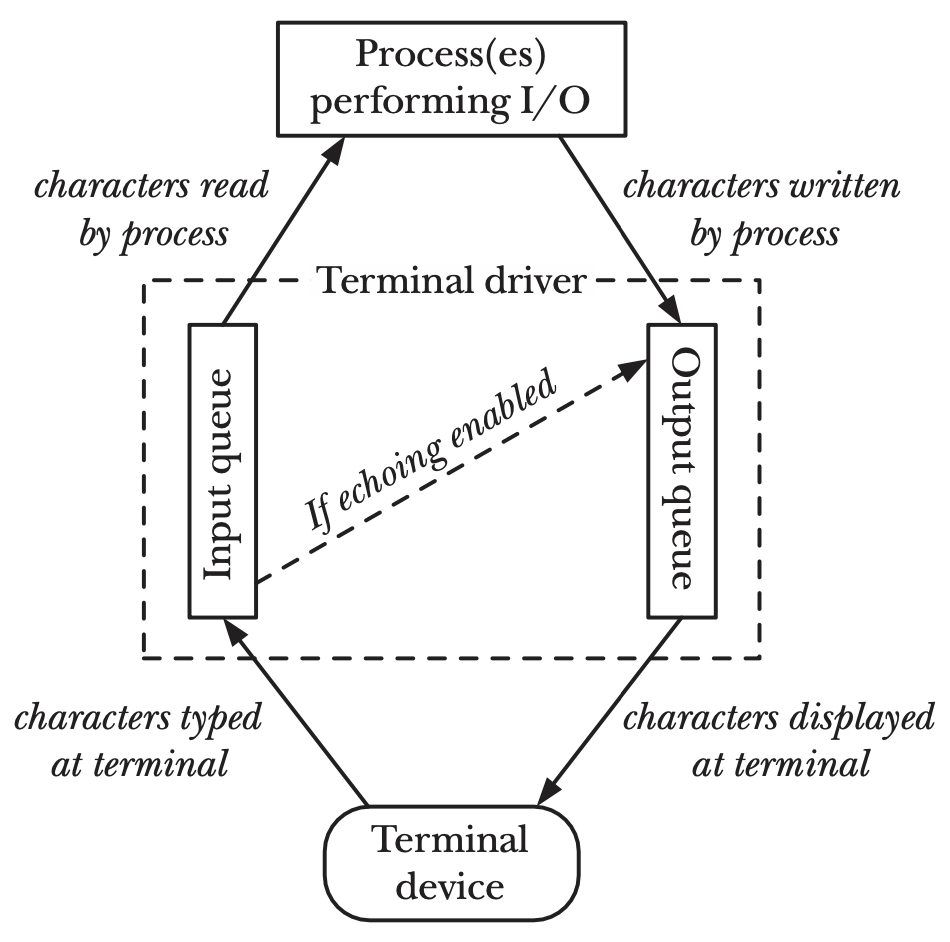
\includegraphics[width=0.8\linewidth]{images/terminal_driver.png}
    \caption{Le fonctionnement d'un pilote de terminal}
\end{figure}

\newpage

\subsubsection{Le mode canonique (coocked mode)}
Ce mode permet au pilote de terminal de traiter les caractères par lignes. La fin d'une ligne est délimitée par le caractère \textbf{newline}.
Quand l'utilisateur presse la touche \textbf{ENTER}, un code ASCII est généré, qui est généralement le code 10. De ce fait, le pilote de terminal sait qu'il faut s'arrêter après ce caractère spéciale et prendre en compte toute la ligne jusqu'au délimiteur.
Une opération de lecture \textbf{read()} sera alors effectuer et la ligne sera retourner au processus. Les caractères spéciaux sont aussi prise en charge sur ce mode.

\subsubsection{Le mode non-canonique (raw mode)}
Ce mode permet au pilote de terminal de traiter une caractère à la fois. Un délimiteur n'est pas utiliser dans ce type de mode, la lecture \textbf{read()} est effectuer directement.
L'outil d'édition de texte comme \textbf{Vi} utilise ce type de mode, les caractères spéciaux ne sont pas prise en charge pour évité toute confusion avec les commandes sur Vi.

\hspace{1cm}

De plus, selon le mode choisi, le pilote de terminal peut aussi traiter les caractères spéciaux.
Les caractères spéciaux peuvent être de 2 types : \textbf{l'édition de l'input} ou \textbf{les signaux}.

\begin{itemize}
    \item Le caractère spécial pour l'édition d'input est par exemple la touche \textbf{DEL}, aussi appelé un caractère \textit{ERASE}.
    \item Le caractère spécial \textit{INTR} correspond généralement à une combinaison de touches \textbf{CONTROL+C} qui va envoyer un signal d'interruption.
\end{itemize}

\hspace{1cm}

\begin{tcolorbox}[colback=white,colframe=example,title=Exemple pour le mode canonique]
    Lorsque un utilisateur tape sur le clavier du texte. Chaque caractère est définis dans un code ASCII.
    Si on tape \textbf{abc}, celui-ci correspond en réalité à \textbf{97 98 99}. C'est donc ces 3 codes qui sont stocker dans le tampon d'entrée.
    Maintenant, pour que le pilote de terminale sache exactement quand s'arrêter et quel ligne retourner, il faut utiliser un caractère spéciale.
    Comme dit précedemment, le caractère spéciale \textit{newline} correspond au code ASCII \textbf{10}.
    Dans le tampon d'entrée, une fois la touche \textbf{ENTER} pressé, le code ASCII \textbf{10} est ajouter à la fin dans le tampon d'entrée.
    Là, le pilote de terminal distingue le délimiteur et effectue une lecture \textit{read()} et renvoie la ligne lue au processus.
\end{tcolorbox}

\begin{tcolorbox}[colback=white,colframe=information,title=Information utile]
Il est possible de modifier les caractéristiques d'un périphérique terminal grâce à l'interface \textbf{termios} sur Linux.
Plusieurs fonctions sont à disposition comme: \textit{tcgetattr} qui permet de stocker les caractéristiques d'un terminal dans une structure à partir de sont descripteur de fichier, et la fonction \textit{tcsetattr} qui permet d'appliquer la nouvelle structure sur le terminal.
Les modifications qu'on peut apporter avec ça est entre autres: modifier le mode du terminal, etc...
\end{tcolorbox}

\newpage

\subsection{L'émulateur de terminal}

L'émulateur de terminal permet de créer une interface textuelle en qui imite le fonctionnement d'un terminal physique.
Tout comme les \textbf{consoles virtuelles}, l'émulateur de terminal utilise les pseudos-terminaux pour créer un canal de communication entre 2 ou plusieurs processus. Lorsqu'un émulateur de terminal est lancé, il initie la création d'une paire de pseudo-terminaux (pty) comprenant un côté maître et un côté esclave. Le côté maître est associé à l'émulateur de terminal lui-même, et le côté esclave est associé à un processus qui tourne le \textbf{bash}.

\begin{figure}[h]
    \centering
    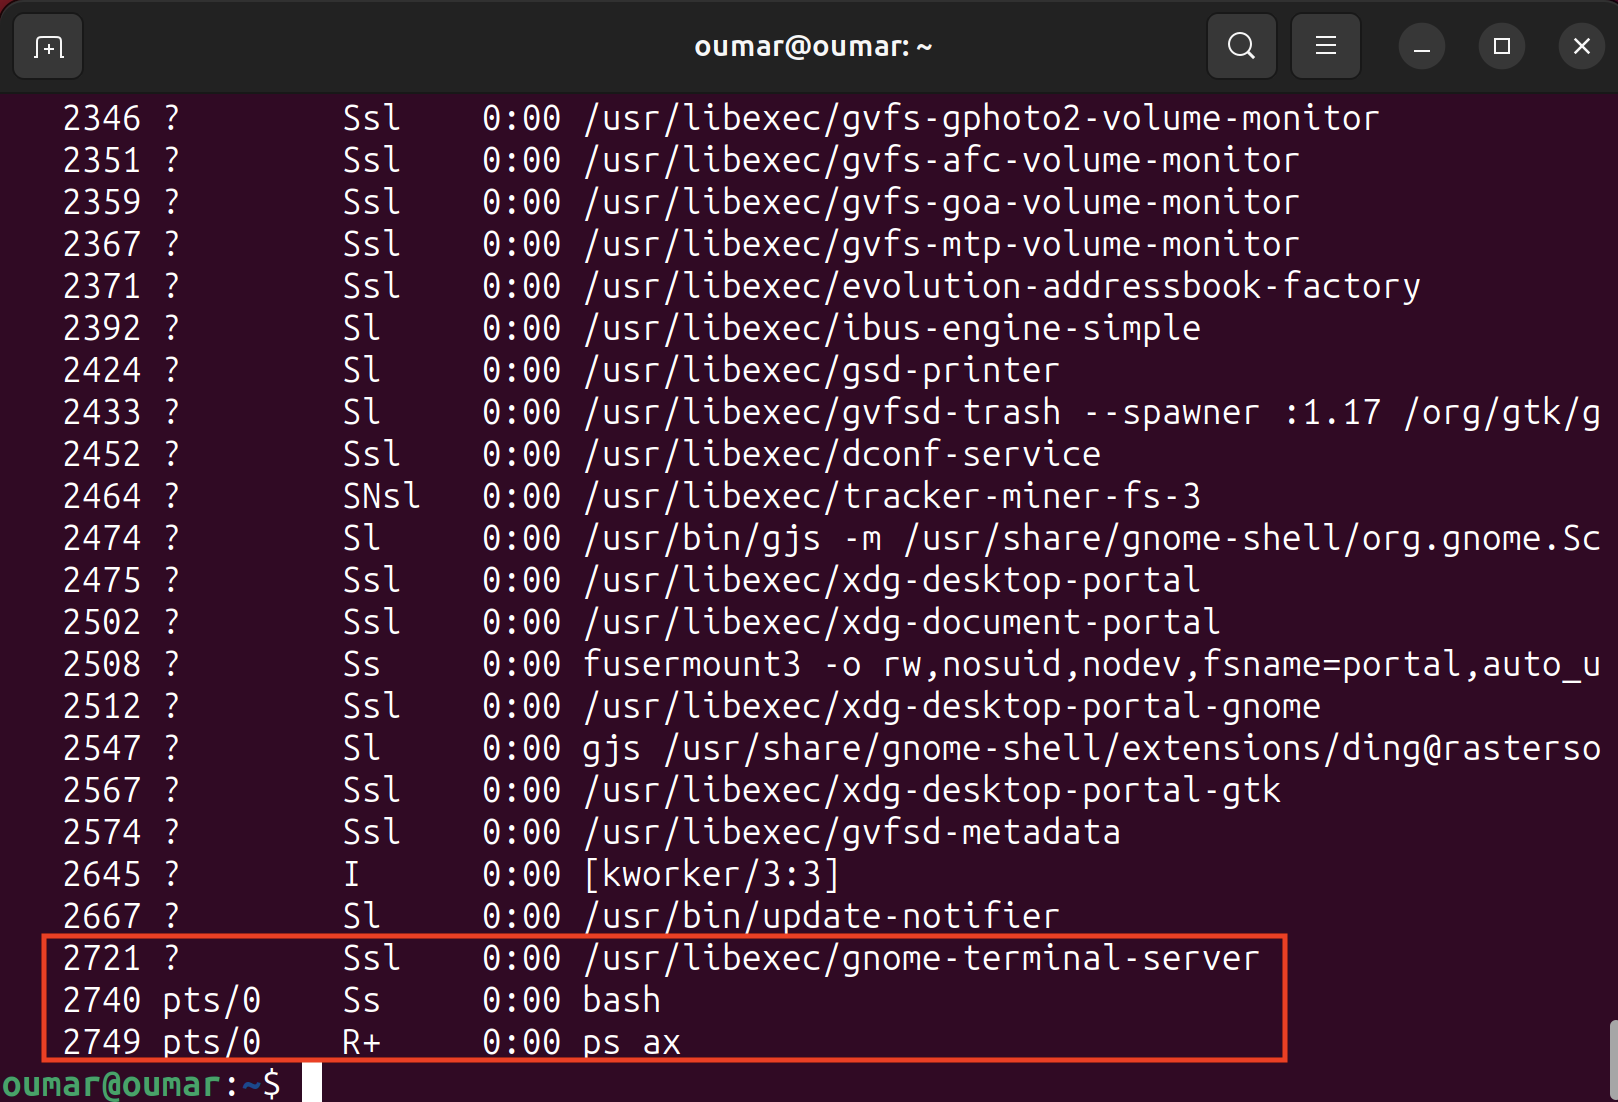
\includegraphics[width=0.8\linewidth]{images/emulator-terminal.png}
    \caption{L'affichage de la commande \textbf{ps ax}}
\end{figure}

Les données entrées passent d'abord par l'émulateur de terminal qui joue le rôle de maître. Une fois les données reçu, elles sont envoyer au côté esclave, qui est le processus qui lance \textbf{bash}.
Une fois que \textbf{bash} a interprété la commande, le retour est renvoyé au côté master depuis le côté esclave. Il y a donc bien une communication bidirectionnelle entre le maître et l'esclave.